%++++++++++++++++++++++++++++++++++++++++
% Don't modify this section unless you know what you're doing!
\documentclass[letterpaper,12pt]{article}
\usepackage{tabularx} % extra features for tabular environment
\usepackage{amsmath}  % improve math presentation

\usepackage{graphicx}
\graphicspath{{images/}}
\usepackage[section]{placeins}

\usepackage[margin=1in,letterpaper]{geometry} % decreases margins
\usepackage{cite} % takes care of citations
\usepackage[final]{hyperref} % adds hyper links inside the generated pdf file
\hypersetup{
	colorlinks=true,       % false: boxed links; true: colored links
	linkcolor=blue,        % color of internal links
	citecolor=blue,        % color of links to bibliography
	filecolor=magenta,     % color of file links
	urlcolor=blue         
}
%++++++++++++++++++++++++++++++++++++++++
\usepackage[UKenglish]{babel}% http://ctan.org/pkg/babel


\begin{document}

\title{What is an isotope?}
\author{Max Sepulveda}
\date{\today}
\maketitle

\begin{abstract}
This paper presents my research on the subject of isotopes. Isotopes that have the same number of protons and electrons, but a different number of neutrons.

\end{abstract}


\section{Isotopes are...}

...atoms that have the same number of protons and electrons, but a different number of neutrons. Changing the number of neutrons in an atom does not change the element. Atoms of elements with different numbers of neutrons are called ``isotopes'' of that element.
\\
Since neutrons have no electrical charge, changing the number of neutrons does not affect the chemistry of the element. It does, however, change the mass of the element. Isotopes are identified by their mass, which is the total number of protons and neutrons.

\begin{itemize}

\item Isotopes are samples of an element with different numbers of neutrons in their atoms.
\item The number of protons for different isotopes of an element does not change.
\item Not all isotopes are radioactive. Stable isotopes either never decay or else decay very slowly. Radioactive isotopes undergo decay.
\item When an isotope decays, the starting material is the parent isotope. The resulting material is the daughter isotope.

\end{itemize}

\pagebreak

\section{Examples of isotopes}

Carbon 12 and Carbon 14 are both isotopes of carbon, one with 6 neutrons and one with 8 neutrons (both with 6 protons). Carbon-12 is a stable isotope, while carbon-14 is a radioactive isotope (radioisotope).

\begin{figure}[!htb] 
        % read manual to see what [ht] means and for other possible options
        \centering 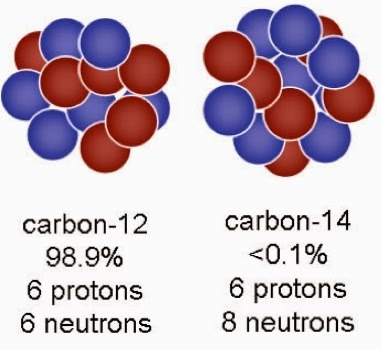
\includegraphics[width=0.3\columnwidth]{main}
        % note that in above figure file name, "sr_setup",
        % the file extension is missing. LaTeX is smart enough to find
        % apropriate one (i.e. pdf, png, etc.)
        % You can add this extention yourself as it seen below
        % both notations are correct but above has more flexibility
        %\includegraphics[width=1.0\columnwidth]{sr_setup.pdf}
        \caption{
                \label{fig:bottle} % spaces are big no-no withing labels
                % things like fig: are optional in the label but it helps
                % to orient yourself when you have multiple figures,
                % equations and tables
                Carbon-12 and Carbon-14 isotopes.
        }
\end{figure}



\begin{thebibliography}{99}

\bibitem{definition}
Isotopes Definition and Examples in Chemistry
    \href{https://www.thoughtco.com/definition-of-isotopes-and-examples-604541}{https://www.thoughtco.com/definition-of-isotopes-and-examples-604541}

\bibitem{favourite}
Chemistry for Kids Isotopes
    \href{https://www.ducksters.com/science/chemistry/isotopes.php}{https://www.ducksters.com/science/chemistry/isotopes.php}

\end{thebibliography}


\end{document}
